\section{State-based invariants through Fluents\label{section:background-fluents}}

Miller and Shanahan define fluents as ``\emph{time-varying properties of the world that are true at particular time-points if they have been initiated by an event occurrence at some earlier time-point, and not terminated by another event occurrence in the meantime. Similarly, a fluent is false at a particular time-point if it has been previously terminated and not initiated in the meantime}''~\cite{Miller:2002}.

Mathematically, a fluent $Fl$ is a proposition defined by a set $Init_{Fl}$ of initiating events, a set $Term_{Fl}$ of terminating events, and an initial value $Initially_{Fl}$ that can be true or false. The sets of initiating and terminating events must be disjoint. The concrete syntax for fluent definition is the following~\cite{Giannakopoulou:2003}:

\begin{center}
fluent $Fl = \textless Init_{Fl}, Term_{Fl} \textgreater $ initially $Initially_{Fl}$
\end{center}

In our train example, the safety goal ``\emph{\texttt{Doors shall remain closed while the train is moving}}'' suggest two fluents defined as follows:

\begin{center}
fluent $Moving = \textless \{start\}, \{stop\} \textgreater $ initially $false$ \\
fluent $DoorsClosed = \textless \{close\}, \{open\} \textgreater $ initially $true$ \\
\end{center}

\subsection{Fluent values along single traces}

Fluents nicely interface with trace semantics as follows. A fluent $Fl$ is said to be $true$ after a finite trace $s$ if and only if one of the following conditions hold~\cite{Giannakopoulou:2003}:

\begin{enumerate}
\item $Fl$ holds initially and no terminating event has occurred in $s$.
\item Some initiating event has occurred in $s$ with no terminating event occurring since then.
\end{enumerate}

Given this definition, for example, the fluent $Moving$ is $true$ after the trace \artifact{<start stop start>}, but not after the empty trace $\lambda$ nor after \artifact{<start stop>}. Note that, as initiating and terminating events are disjoint, the value of a fluent after a given trace is deterministic. Also, taking trace prefixes into account, it is straightforward to think in terms of fluent values \emph{along} traces by rephrasing the above definition as a recursive version~\cite{Damas:2005}. This is illustrated in Fig.~\ref{image:fluent-values-along-a-trace} where the values of the two fluents given above are shown in the states of a LTS modeling a typical event trace for the train system. 

\begin{figure}[H]\centering
\scalebox{0.45}{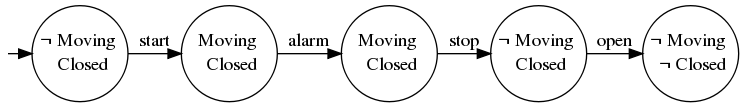
\includegraphics{src/2-framework/images/decorating-trace}}
\caption{Fluent values along a single trace, captured with a LTS. Here \artifact{DoorsClosed} is abbreviated as \artifact{Closed}.\label{image:fluent-values-along-a-trace}}
\end{figure}

As the example suggests, given a set of fluents $\Phi$, a trace (and any of its prefixes) defines an interpretation over $2^\Phi$, that is the assignment of a boolean value to each fluent in $\Phi$. We call them \emph{fluent value assignments} throughout this thesis. For example, the (maximal) trace in the figure defines the assignment $\{Moving \rightarrow false,~DoorsClosed \rightarrow false\}$. 

\subsection{Fluent values along multiple traces}

Interestingly, previous results can be generalized for annotating states of any LTS. The generalization consists in considering that a LTS state may be reached by a set of traces instead of a single one. Therefore annotations become \emph{sets} of fluent assignments, that is elements of $\mathcal{P}(2^\Phi)$. In particular, a state could be reached by a trace rendering a fluent $true$, while another trace reaching it would render the same fluent $false$. Remark however that even in presence of a possibly infinite number of traces, the set of all possible annotations is itself finite. Moreover, $\mathcal{P}(2^\Phi)$ actually coincides with the set of propositional formula over fluents. In fact, it is convenient to interpret state annotations as such formula, where $false$ then corresponds to an empty set of fluent assignments (i.e. an unreachable state) and \artifact{true} corresponds to the set of all possible assignments. We call those state annotations \emph{fluent invariants}, as they encode assertions that always hold when the LTS state is visited. An example is given in Fig.~\ref{image:fluent-values-along-multiple-traces}.

\begin{figure}[H]\centering
\scalebox{0.45}{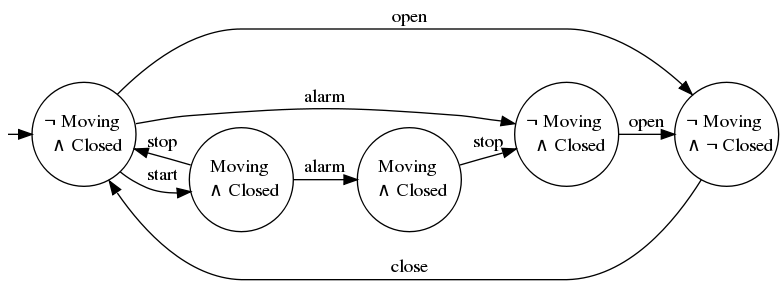
\includegraphics{src/2-framework/images/decorating-lts}}
\caption{Fluent values along multiple traces. Here \artifact{DoorsClosed} is abbreviated as \artifact{Closed}.\label{image:fluent-values-along-multiple-traces}}
\end{figure}

A fix-point algorithm for decorating a LTS with fluent assignments first appeared in~\cite{Damas:2005}; it is generalized for handling state invariants in \cite{Damas:2009}. In short, it consist in annotating the LTS initial state with an initial invariant, according to fluent initial values. Invariants are propagated along LTS transitions, according to fluent definitions and accumulated in states through boolean disjunction until a fix point is reached. One can profit from binary decision diagrams~\cite{Bryant:1986} for concisely encoding and efficiently manipulating boolean formula in an implementation. This algorithm is generalized once again in~\cite{Damas:2011} to work on guarded LTS (see chapter~\ref{chapter:deductive}) as well as for handling other kinds of decorations than state invariants.

\subsection{Integrating fluents in multi-view models}

Fluents, as described in the previous section, provide a general mechanism for interfacing event-based models with state-based abstractions. In this section, we restrict our own use of this mechanism so as to cleanly interface with agents, their state machines, and scenarios. The next section naturally extends this discussion by introducing fluent-based goals and domain properties in the framework.

First of all, we restrict our use of fluents to those \emph{monitored} and \emph{controlled} by the agents forming the system. A fluent is monitored by an agent if all its initiating and terminating events are either sent or received by this agent; it is controlled if all initiating and terminating events are sent by the agent. Considering only monitored and controlled fluents is motivated by the need for state machines and goals to be realizable by their agents~\cite{Letier:2002} (see also next section).

We have seen in the previous section that the value of a fluent is not necessarily known in a LTS state because some traces could render it $true$ while others could render it $false$. While there is no strong agreement for viewing this as problematic in general, we consider a good practice not to fall in such a situation between the fluents monitored and controlled by an agent and the state machine modeling its behavior. The reason is that LTSs are not considered a structured form of state machines. Therefore, a LTS state should not be viewed as a class of agent states, that is, it should correspond to a unique assignment of agent state variables; fluents are such variables. The LTS state machine shown in Fig.~\ref{image:fluent-values-along-multiple-traces} respects this sane property. In particular, one can check that propositional formula shown in states are satisfiable by only one interpretation (fluent invariants ``degenerate'' to fluent value assignments). In such a case, an agent state uniquely defines the value of its monitored and controlled fluents (this property is conserved under LTS composition by construction). T;he contrapositive of this property is not true: as illustrated in the same figure, fluent value assignments do not necessarily identify LTS states.

Following previous assumptions and results, MSC timelines can easily be annotated with agent invariants on monitored and controlled fluents. However note that, as with LTSs, these invariants do not necessarily identify agent states in a unique manner.
